\documentclass[12pt, a4paper, oneside,bibend=bibtex]{ctexart}
\usepackage{fancyhdr}

\usepackage[top=1in, bottom=1in, left=1.25in, right=1.25in]{geometry} 
\usepackage{amsmath, amsthm, amssymb, appendix, bm, graphicx, hyperref, mathrsfs}
\usepackage{pdfpages}
\usepackage{booktabs}
\usepackage{url}
\usepackage{graphicx}
% \pagestyle{plain}
\pagestyle{fancy}
\fancyhead[L]{软件测试实验报告}
\fancyhead[R]{\leftmark}
\fancyfoot[C]{\thepage} % 显示页码

\usepackage{graphicx}  %插入图片的宏包
\usepackage{float}  %设置图片浮动位置的宏包
\usepackage{subfigure}  %插入多图时用子图显示的宏包
\usepackage{dirtree}

\setmainfont{Times New Roman}   %衬线字体缺省英文字体.serif是有衬线字体sans serif无衬线字体
\setmonofont{Courier New}

% \setCJKmainfont{FandolSong-Regular} % 设置正常体字体
% \setCJKsansfont{FandolHei-Regular} % 设置无衬线字体
% \setCJKmonofont{FandolFang-Regular} % 设置等宽字体



\hypersetup{
	colorlinks=true,
	linkcolor=black,
	filecolor=blue,      
	urlcolor=blue,
	citecolor=cyan,
}
\usepackage{titlesec}
\usepackage{listings}
\usepackage{xcolor}


\titleformat*{\section}{\zihao{3}\heiti}
\titleformat*{\subsection}{\zihao{-3}\heiti}
\titleformat*{\subsubsection}{\zihao{4}\heiti}


\linespread{1.5}
\setlength{\parskip}{2ex} % 设置段距为2ex
\newtheorem{theorem}{定理}

\usepackage[most]{tcolorbox}
\definecolor{mygray}{RGB}{240,240,240}
\newtcolorbox{myquote}{%
    colback=mygray,
    colframe=gray,
    boxrule=0pt,
    arc=3mm,
    outer arc=3mm,
    top=8pt,
    bottom=8pt,
    left=10pt,
    right=10pt,
    fontupper=\small,
    drop shadow=gray!50!white,
    before skip=5mm,
    after skip=5mm,
    boxsep=5mm,
    lefttitle=15mm,
    titlerule=1mm,
    breakable % 允许跨页      
}




\begin{document}
% \includepdf{cover.pdf}
% \definecolor{codegreen}{rgb}{0,0.6,0}
% \definecolor{codegray}{rgb}{0.5,0.5,0.5}
% \definecolor{codepurple}{rgb}{0.58,0,0.82}
\definecolor{backcolour}{RGB}{255,254,255}


\renewcommand{\lstlistingname}{Code}
% \renewcommand{\thelstlisting}{\arabic{lstlisting}}

\lstset{
    language=Python,
    language=sh, % 添加shell脚本语言
    backgroundcolor=\color{backcolour}, % 代码块背景色
    captionpos=t, %代码标题位置
    frame=shadowbox, % 代码块边框
    framesep=4pt, % 阴影框和代码框的间距
    rulesepcolor=\color{red!20!green!20!blue!20},%代码块边框为淡青色
    keywordstyle=\color{blue!80!black}\bfseries, % 蓝色加粗关键字
    commentstyle=\color{green!60!black}\itshape, % 绿色斜体注释
    stringstyle=\color{red!70!black}, % 红色字符串
    showstringspaces=false, % 不显示字符串中的空格
    numbers=left, % 显示行号
    numberstyle=\small\ttfamily\color{gray!50}, % 灰色行号,等宽字体
    breaklines=true, % 自动换行
    tabsize=4, % tab大小
    basicstyle=\small\ttfamily, % 等宽字体
    captionpos=t, % 标题在上方
    escapeinside={\%*}{*}, % 包含中文时使用
    extendedchars=true, % 支持中文
    literate={×}{{$\times$}}1 {÷}{{$\div$}}1, % 支持 × 和 ÷ 符号
    morekeywords={as, None, with, yield} % 新增关键字
}




\pagenumbering{roman} % 使用罗马数字页码
\tableofcontents
\hypersetup{
	colorlinks=true,
	linkcolor=blue,
	filecolor=blue,      
	urlcolor=blue,
	citecolor=cyan,
}
\newpage

\pagenumbering{arabic} % 使用阿拉伯数字页码






% \section{操作指南}

% \subsection{代码的插入}
% 代码的插入有两种方式,

% \subsubsection{第一种代码插入方式}
% 第一种是直接输入代码,这样适合直接进行解释代码,这样如果不想输入标题,caption=\{\}即可,如下代码:
% \begin{lstlisting}[caption={}]
% echo "Test"   #This is a shell command
% a+=1
% a="123"
% return 213
% \end{lstlisting}


% \subsubsection{第二种代码插入方式}
% 第二种是引入文件的方式,更多的是把完整的代码文件引入进来,这样最好起一个标题,在caption选项里面起名字即可,如代码 \ref{第二种注释}所示

% % 两种代码的输入方式
% \lstinputlisting[caption={第二种注释代码的方式}, label={第二种注释}]{code/generateHandleOnce.py}


% \subsection{引用块的使用}

% 在对一些代码进行官方的解释时,需要以引用块的形式括上官方解释,如下。根据Gcov的定义\footnote{\url{https://www.tutorialspoint.com/unix_commands/gcov.htm}}。
% \begin{myquote}
% gcov是GNU代码覆盖率测试工具。它是一个命令行工具,用于测试C、C++和Fortran程序的代码覆盖率。gcov可以用于计算每个源代码行被执行的次数,并为程序中每个函数提供一个覆盖率分数。gcov生成的输出可以用于检测代码中的未测试部分,以及对测试的优化。
% \end{myquote}
% 并且,与插入代码是类似的,myquote支持跨页,因此不用像图片和表格一样担心跨页的问题。

% \textbf{解释:参考上面这个网址,最好在说明一个命令的时候,先引用一下网址再采用quote块。采用脚注的方式引用,不用cite引用(放刚刚那个网址就可以了,不一定非要网址内容和引用块中的内容对应,但是放的网址还是要稍微正规一点)。总的来说就是先footnote网址,然后再用myquote稍微解释一下,具体代码格式如下}:
% \begin{myquote}
% \begin{verbatim}
% 如下。根据xxx的定义\footnote{\url{https://www.}}。
% 网址就采用刚刚那个就可以了,搜一个命令换一个网址
% \begin{myquote}
% xxxx
% \end{myquote}
% \end{verbatim}
% \end{myquote}


% % \subsection{表格}
% % 表格采用三线表格式,如表 \ref{测试表格}。但是似乎这个报告不太需要表格?
% % \begin{table}[htbp]
% %     \centering
% %     \caption{这是一个三线表的例子} \label{测试表格}
% %     \begin{tabular}{lcr}
% %         \toprule[2pt]
% %         \textbf{姓名} & \textbf{年龄} & \textbf{性别} \\
% %         \midrule[1pt]
% %         张三 & 22 & 男 \\
% %         李四 & 28 & 男 \\
% %         \bottomrule[2pt]
% %     \end{tabular}
% % \end{table}




\section{引言}
当今的软件开发越来越复杂,需要应对不同的需求和场景,因此测试也变得越来越重要\cite{khan2014importance}。测试不仅是为了发现软件中的错误和漏洞,也是为了保证软件的正确性、可靠性和稳定性。在测试过程中,测试用例的设计和编写是非常关键的,它们需要覆盖软件中的所有可能情况,以确保软件的正确性和可靠性。除了测试用例,还有一些测试方法和工具可以帮助开发者在软件开发和测试中提高效率和质量。

白盒测试是一种常用的测试方法,它需要开发者深入了解代码的内部实现,通过分析代码的执行路径来设计测试用例。与黑盒测试不同,白盒测试可以检测到软件中的逻辑错误和边界条件问题,因此在软件开发和测试中非常有用\cite{bertolino2007software}。然而,白盒测试需要开发者具备较强的编程和测试技能,需要大量的时间和精力来设计和编写测试用例。

自动化测试工具是另一个可以提高测试效率和质量的工具。自动化测试可以帮助开发者快速执行大量的测试用例,检测软件中的错误和漏洞,并生成详细的测试报告。自动化测试可以减少测试的时间和人力成本,提高测试的覆盖率和质量\cite{myers2011art}。

gcov 是一个常用的代码覆盖率分析工具,它可以帮助开发者分析代码的覆盖率,找到未经测试的代码,并提高代码的质量和可靠性。通过 gcov 生成的代码覆盖率报告可以告诉开发者哪些代码没有被测试到,以及哪些测试用例可以增加代码覆盖率。这些信息可以帮助开发者设计更好的测试用例,提高测试的覆盖率和质量。同时,gcov 也可以帮助开发者发现代码中的漏洞和错误,从而提高软件的质量和可靠性\cite{pezze2008software}。

在本实验中,我们将学习如何使用 gcov 命令来生成代码覆盖率报告,并通过分析报告来发现代码中的漏洞和错误。通过实践和分析,我们将掌握一些软件测试的相关方法和经验,例如,如何设计和编写高质量的测试用例,如何进行白盒测试,以及如何使用自动化测试工具来提高测试效率等。

\subsection{实验目的}
\begin{enumerate}
    \item[(1)] 利用gcov对待测试项目进行自动化测试并分析可以帮助我们了解代码的覆盖率情况,发现未经测试的代码,从而提高代码的质量和可靠性。通过这个实验,我们可以学习如何使用gcov命令来生成代码覆盖率报告,并通过分析报告来发现代码中的漏洞和错误。
    
    \item[(2)] 通过对测试结果的分析,我们可以掌握一些软件测试的相关方法和经验。例如,我们可以了解如何设计和编写高质量的测试用例,如何进行白盒测试,以及如何使用自动化测试工具来提高测试效率等。这些经验对于我们在软件开发和测试中都非常有用,可以帮助我们提高软件质量和可靠性,减少开发成本和时间。
\end{enumerate}
\subsection{实验原理}
\subsubsection{白盒测试}
\begin{figure}[ht]
    \centering
    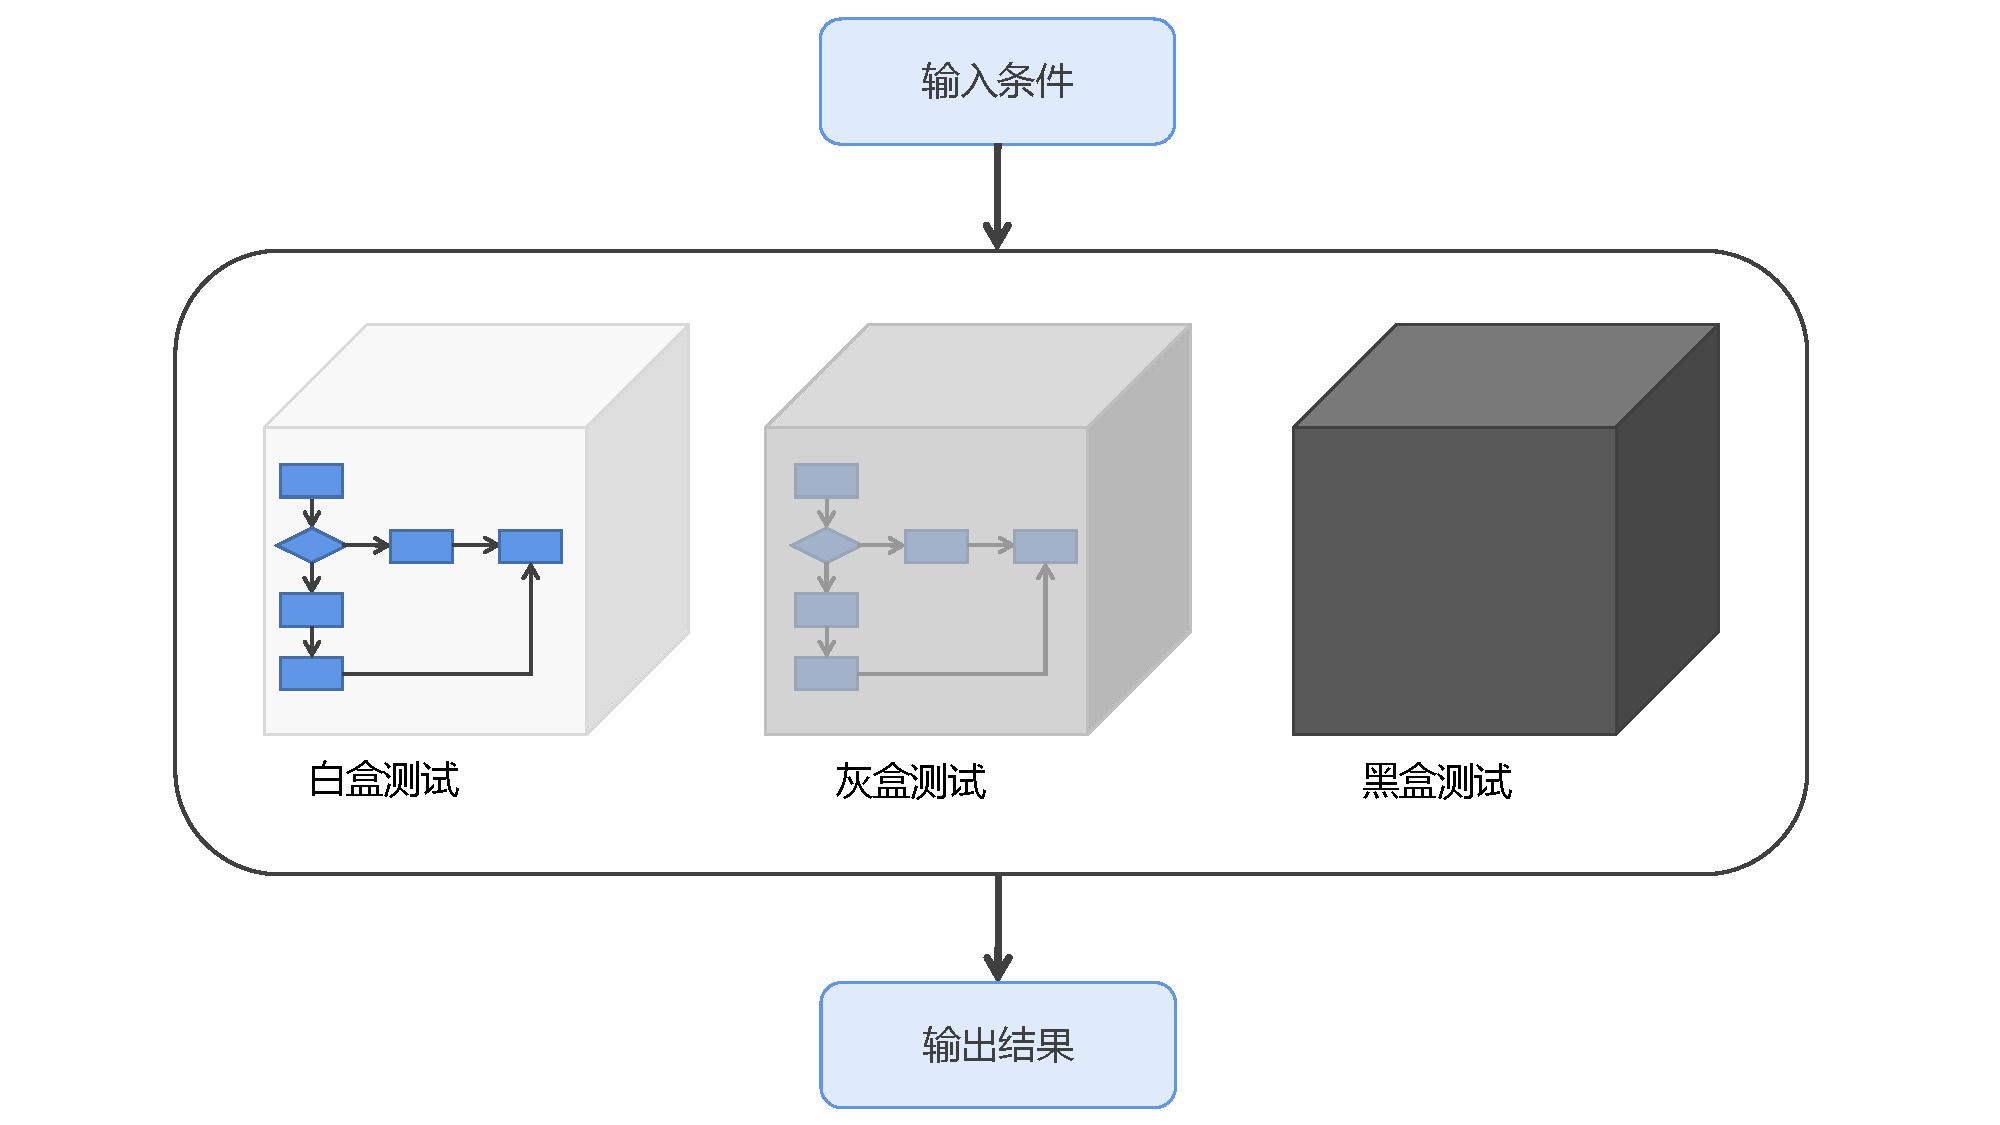
\includegraphics[width=1\linewidth]{images/white_test.pdf}
    \caption{白盒测试需要深入分析内部结构}
    \label{white}
\end{figure}
白盒测试(White-box testing)是一种软件测试方法,也称为结构测试或基于代码的测试。它基于深入了解软件系统的内部结构和工作原理来测试软件系统的正确性、可靠性和健壮性。在白盒测试中,测试人员通常需要访问和分析软件系统的源代码,以确定测试案例的范围和内容。测试人员可以使用各种技术和工具来检查代码,例如\textbf{代码覆盖率分析、路径分析、逻辑覆盖测试}等。

如图\ref{white}所示,白盒测试可以帮助测试人员了解软件系统的内部结构和工作原理,以便更好地识别和修复软件系统中的缺陷。此外,白盒测试还可以帮助测试人员确定哪些代码需要更多的测试覆盖和哪些代码不需要测试覆盖。
\subsubsection{语句覆盖}
语句覆盖(Statement coverage)是一种软件测试技术,它的目的是测试程序中的每个语句是否至少被执行一次。在语句覆盖测试中,测试人员编写测试用例并执行这些测试用例来测试程序。在执行测试用例的过程中,测试人员记录下执行的语句,最终确定是否覆盖了所有的语句。如果所有的语句都被执行了至少一次,那么语句覆盖就达到了100\%。

语句覆盖测试可以帮助测试人员发现程序中未被执行的语句,从而减少程序中的漏洞和缺陷。但是,语句覆盖测试并不能保证程序的完全正确性,因为它并没有测试程序中语句之间的关系和逻辑正确性。需要注意的是,在进行语句覆盖测试时,测试人员应该注意测试用例的质量和覆盖率,尽可能地覆盖所有可能的情况,以便发现程序中的潜在问题。
\subsubsection{分支覆盖}
分支覆盖(Branch coverage)是一种软件测试技术,它的目的是测试程序中的每个分支是否都被执行至少一次。在分支覆盖测试中,测试人员编写测试用例并执行这些测试用例来测试程序。在执行测试用例的过程中,测试人员记录下执行的分支,最终确定是否覆盖了所有的分支。如果所有的分支都被执行了至少一次,那么分支覆盖就达到了100\%。

分支覆盖测试可以帮助测试人员发现程序中未被执行的分支,从而减少程序中的漏洞和缺陷。与语句覆盖测试不同的是,分支覆盖测试还可以测试程序中的分支之间的关系和逻辑正确性。需要注意的是,在进行分支覆盖测试时,测试人员应该注意测试用例的质量和覆盖率,尽可能地覆盖所有可能的情况,以便发现程序中的潜在问题。
\subsubsection{实验团队信息}
小组组长:XX

小组成员:XX, XX, XX, XX, XX
\section{实验配置}




\subsection{硬件设备} 
该实验在提供的虚拟镜像下完成:如图\ref{硬件}所示,当前系统的版本为Ubuntu 21.04。其他硬件信息如内存分配等完全与镜像配置一致。
\begin{figure}[htbp]
    \centering
    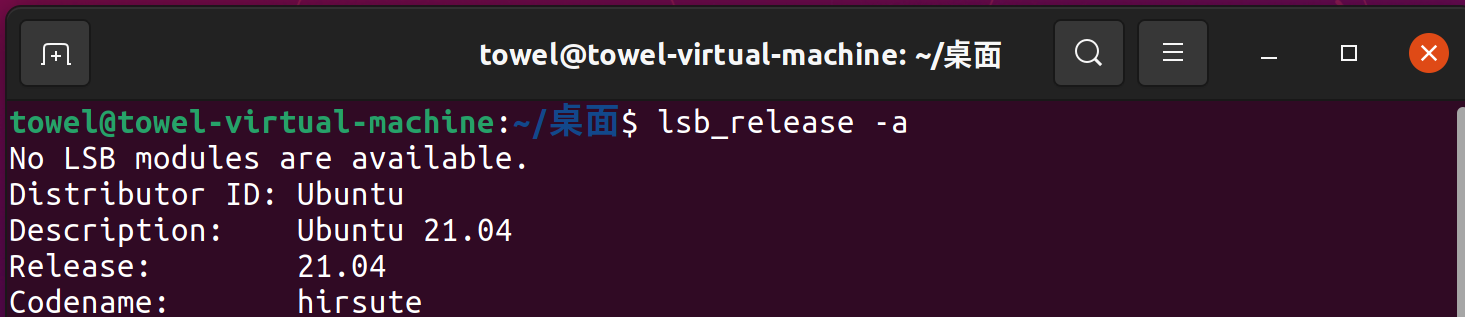
\includegraphics[width=0.9\linewidth]{images/hardware.png}
    \caption{实验运行操作系统配置}
    \label{硬件}
\end{figure}
\subsection{软件配置} 
\begin{enumerate}
    \item 对于自动化运行代码的编辑工具,我们主要是在VS Code(v1.76.1)中完成。
    \item 对于Shell类型,我们除了在Linux原生Shell终端中进行操作之外,还利用了VSCode的终端中进行操作。从图\ref{原生shell}和图\ref{Vsshell}中可以看出,两种终端都是运行的Bash作为命令行解释器。

\begin{figure}[htbp]
	\centering  %图片全局居中
	\subfigure[原生终端Shell类型]{
		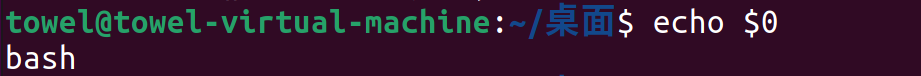
\includegraphics[width=0.8\linewidth]{images/shellV.png}
  \label{原生shell}}
	\subfigure[VSCode终端Shell类型]{
		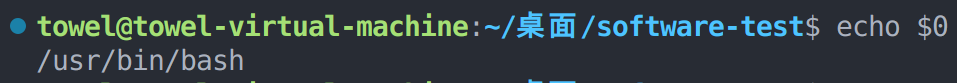
\includegraphics[width=0.8\linewidth]{images/vscV.png}
  \label{Vsshell}}
	\caption{两种Shell类型比较}
 \end{figure}
    \item 对于生成自动化脚本的工具,我们使用Python语言(v3.9.4)。在第\ref{脚本选择章节}章节中,会对该工具以及自动化生成脚本的过程进一步介绍。
    \item 对于小组代码提交工具,我们采用Git来进行分布式版本控制。如图\ref{git}所示,我们的核心代码在Master主分支上的提交记录呈现如图。为了方便小组合作,我们采用Gitee进行代码托管。这样所有成员就可以随时进行代码版本更新与资源同步。
    \begin{figure}[htbp]
    \centering
    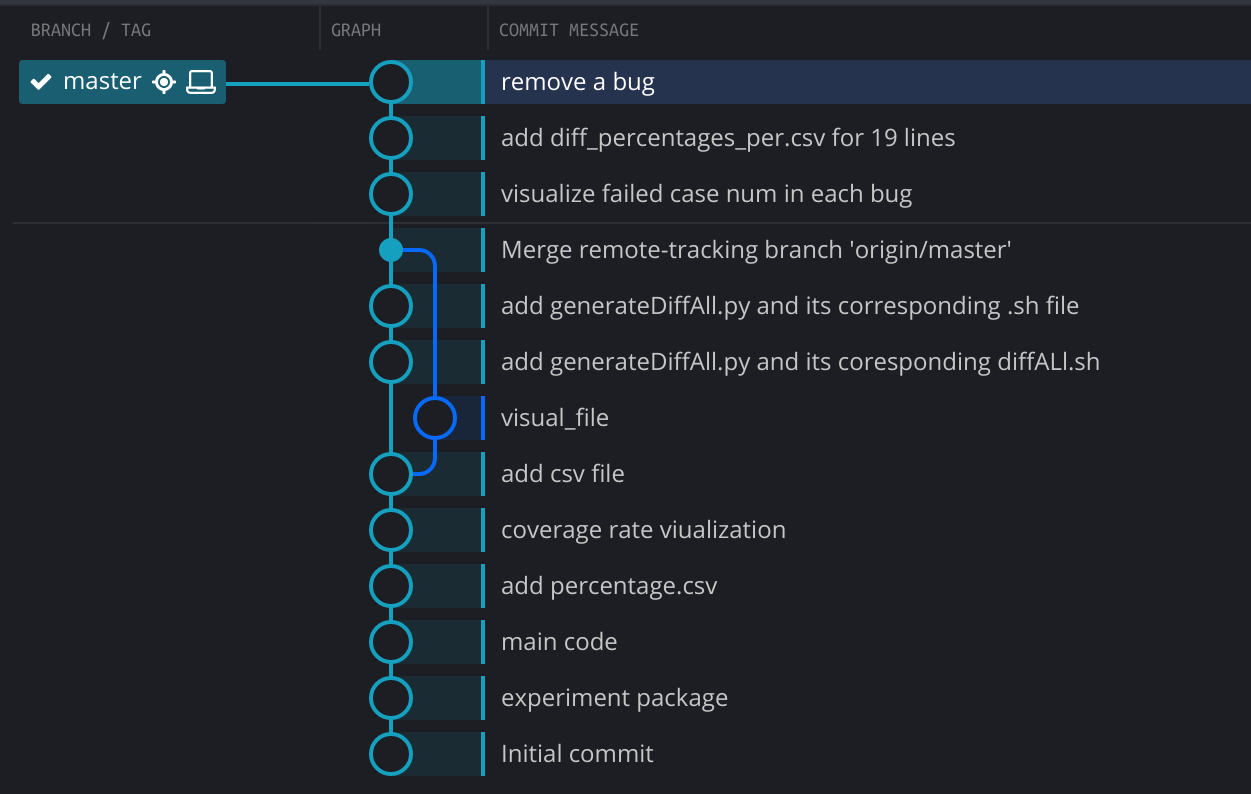
\includegraphics[width=0.8\linewidth]{images/git.png}
    \caption{实验代码版本管理}
    \label{git}
\end{figure}


\end{enumerate}


\subsection{文件目录结构}
对于整个项目目录$Project$,总体采用如下的分布:
\dirtree{%
.1 Project.
.2 grep\_1.2.
.3 grep.
.2 SourceCode.
.3 pySourceCode.
.4 processCode.
.5 generateHandle.
.5 generateDiff.
.4 ShellCode.
.4 extractDataCode.
.2 visualizeCSV.
}
对于grep\_1.2,实际就是实验提供的源代码,包含了需要进行测试分析的程序。第二部分是我们编写的自动化测试代码的集合,其中生成类代码分为生成插桩覆盖的代码和生成输出结果对比的两类测试处理代码;还包括生成出Shell代码以及最后的数据提取代码。最后是提取出数据的csv文件的集合,便于在第\ref{实验章节}章节的后续进行数据分析。


\section{实验}\label{实验章节}

\subsection{总体架构}
如图\ref{实验流程图}所示,本次实验总共可以从宏观上划分为4个板块:实验预处理、实验计划实施、自动化测试和可视化分析。从细节步骤上:首先我们了解了核心指令含义以及对输入用例进行预处理;然后通过从单次覆盖到多次覆盖,以及从语句覆盖到分支覆盖来层层递进,实施了实验计划;通过自动化编写脚本:完成了18个Bug的测试覆盖,并对Gcov插桩输出的内容与Test Oracle进行对比;最后,我们还编写了脚本提取总结出实验过程中的核心数据,并完成了可视化分析。

\begin{figure}[htbp]
    \centering
    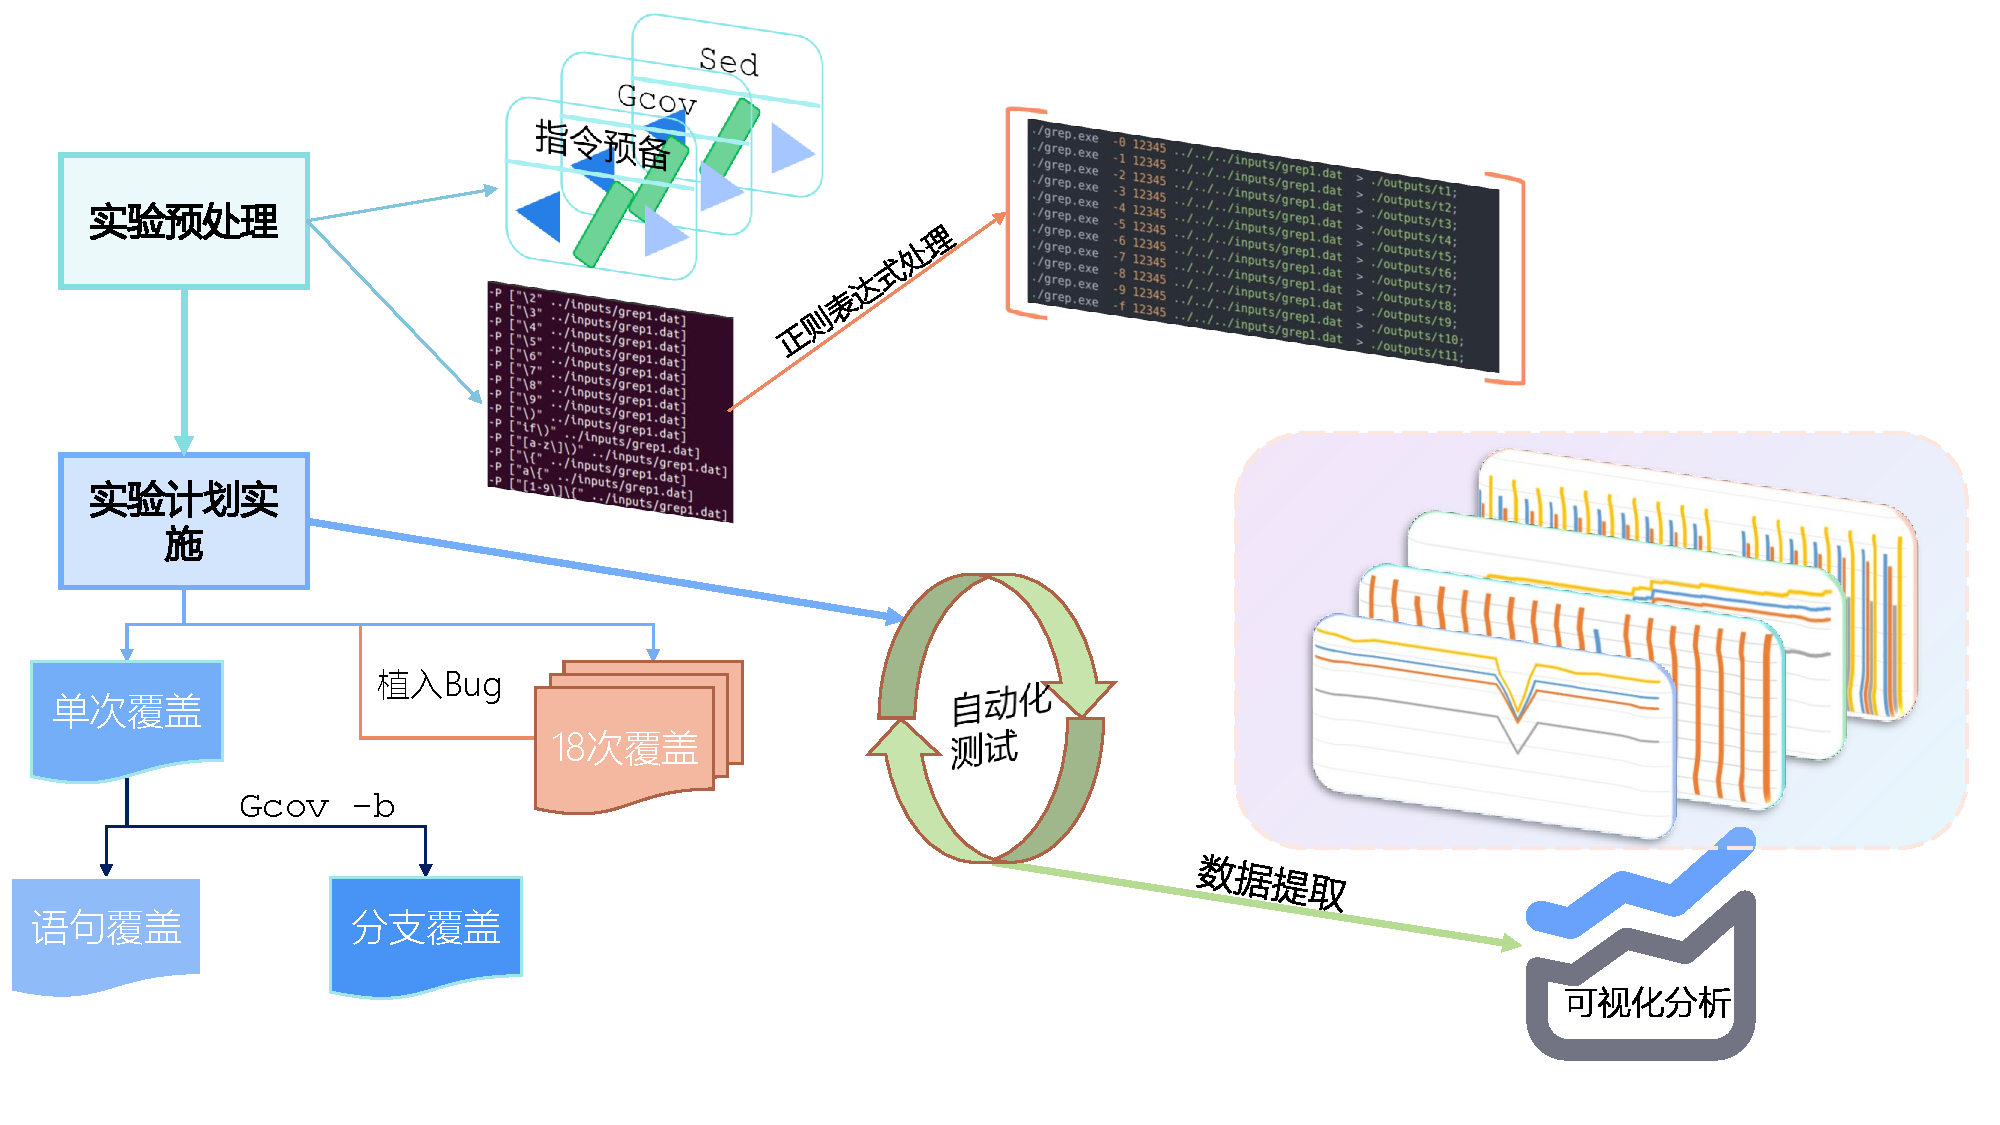
\includegraphics[width=1\linewidth]{images/exp_pro.pdf}
    \caption{实验整体流程}
    \label{实验流程图}
\end{figure}

\subsection{脚本语言选择} \label{脚本选择章节}
在本次实验中,我们需要自动化地执行大量的测试用例并分析测试结果。我们根据实验本身的特点,利用Shell脚本进行输入数据与测试。对于$18$个插入的Bug,每一个Bug都要经过一轮$199$个用例的完整测试,并且输出到不同的文件夹下。因此手动输入这$199\times 18=3582$个用例是极其费力的,也不符合自动化测试的思想。因此,为了实现自动化测试这一目标,我们选择了两种脚本语言:Shell脚本和Python脚本。这两种脚本语言各自具有独特的优势,使我们能够更有效地完成实验任务。
\begin{enumerate}
    \item \textbf{Shell脚本:}
    \begin{itemize}
        \item Shell脚本在处理文件操作和系统命令方面具有优势,使我们能够轻松地执行用例并将结果输出到不同的文件夹下。
        \item Shell脚本可以直接在实验环境的Ubuntu操作系统的Shell中运行,方便快捷。
        \item Shell脚本在执行简单任务时性能较好,适合我们实验中的大部分操作。
    \end{itemize}
    \item \textbf{Python脚本:}
    \begin{itemize}
        \item Python具有丰富的内置库和第三方库。这使得Python在处理字符串和文件读写方面非常强大。
        \item Python具有简洁明了的语法,易于编写和阅读。
        \item Python具有很好的跨平台兼容性,我们对Python代码的编写与测试既可以在本地电脑,也可以在虚拟机中进行。
    \end{itemize}
\end{enumerate}
在实验过程中,我们首先使用Python脚本生成$.sh$类型的Shell脚本文件,以便自动执行所有测试用例。之后,我们使用Python脚本对测试结果进行提取、处理和分析,生成$.csv$文件以便进行数据可视化。这种脚本语言选择策略的优势在于充分利用了Shell脚本和Python脚本各自的优势,提高了实验效率;同时,使实验过程更加自动化,减少了人为错误的可能性;并且,这还便于后期实验结果的分析和可视化,提高了实验的可读性和准确性。


\subsection{实验预处理}
在正式开始编写测试脚本和执行测试代码之前,我们需要对实验做一些预处理,包括测试用例命令的纠正、Bug的植入并编写Python代码完成这些预处理。图\ref{process}展示了实验预处理工作的组织结构。

\begin{figure}[htbp]
    \centering
    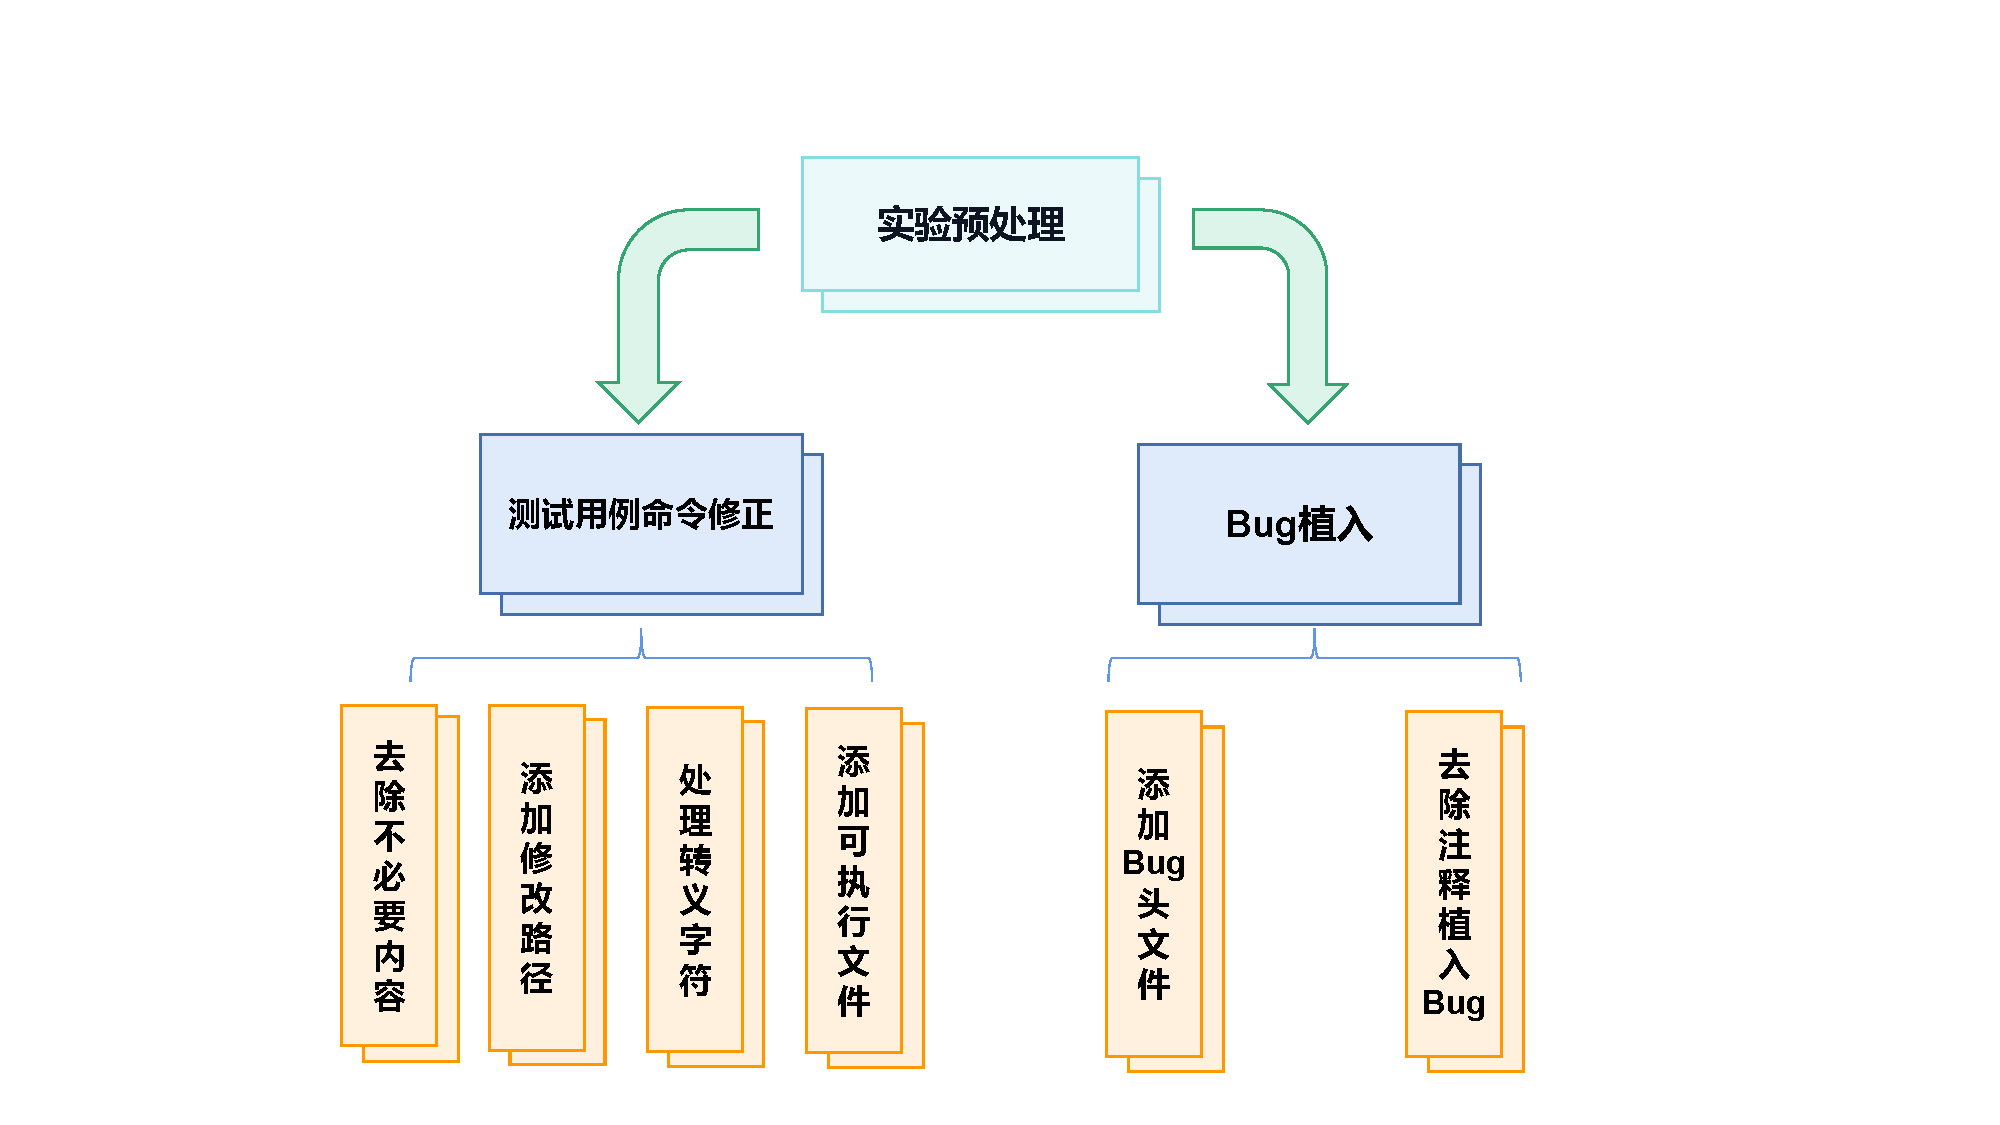
\includegraphics[width=16cm]{images/handle.pdf}
    \caption{实验预处理整体架构}
    \label{process}
\end{figure}

\subsubsection{测试用例命令修正}
本次实验的测试用例命令存储在$testplans.alt/v1$目录下的$v0.cov.universe$中。如图\ref{universe}所示,我们需要对其做出如下修改以便测试用例可以正确执行:
\begin{itemize}
    \item \textbf{删除命令中的“-P”参数。} 图\ref{universe}所示的每一行测试用例命令皆以-P开头,这在实际执行测试代码时是不需要的,我们将其删除。
    \item \textbf{删除非输入内容中的中括号。} 同时,每行测试用例命令都由“[ ]”包围,这在实际执行测试代码时同样不需要,但其中的个别用例输入本身包含"["或"]",这些符号需要保留,否则就改变了原本的测试用例。因此,我们需要在删除不必要中括号的同时不改变测试输入里的中括号。
    \item \textbf{修改测试用例命令中的目录。} 在我们的实验目录结构中,$grep1.dat$文件处在$grep/inputs/$目录下,与测试用例命令中的$../inputs/$不符,需要改正。
    \item \textbf{处理测试用例中的转义字符。} 由于部分测试用例输入中含有“$\backslash$”符号,而这在Shell脚本语言中会被理解为转义字符,因此我们需要在“$\backslash$”前添加转义字符使其能够被正确理解为符号本身。
    \item \textbf{添加可执行文件的命令。} 要正确执行测试代码,我们需要在每行测试用例命令前添加可执行文件名$./grep.exe$。
    \item \textbf{添加测试结果输出路径。} 由于最终需要对测试代码的执行结果进行分析比对,因此我们为每次测试的执行结果指定各自的输出路径。
\end{itemize}

\begin{figure}[htbp]
    \centering
    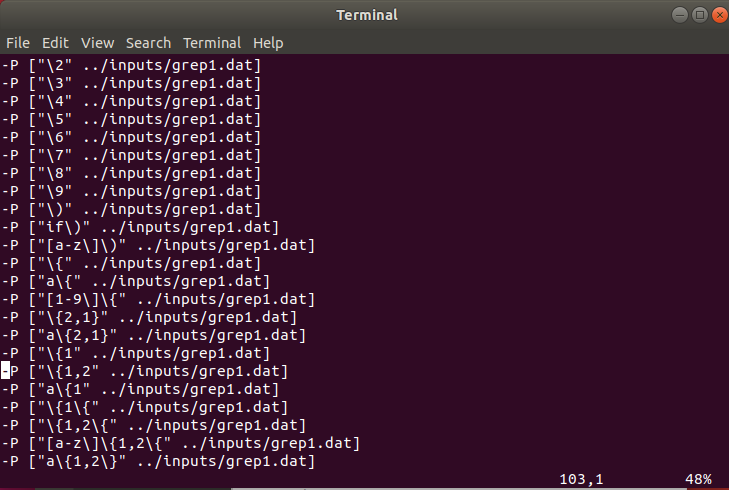
\includegraphics[width=14cm]{images/universe.png}
    \caption{v0.cov.universe中的测试用例}
    \label{universe}
\end{figure}

\subsubsection{Bug植入}
我们在$grep.c$文件添加$FaultSeeds.h$头文件以植入Bug。
\begin{figure}[htbp]
    \centering
    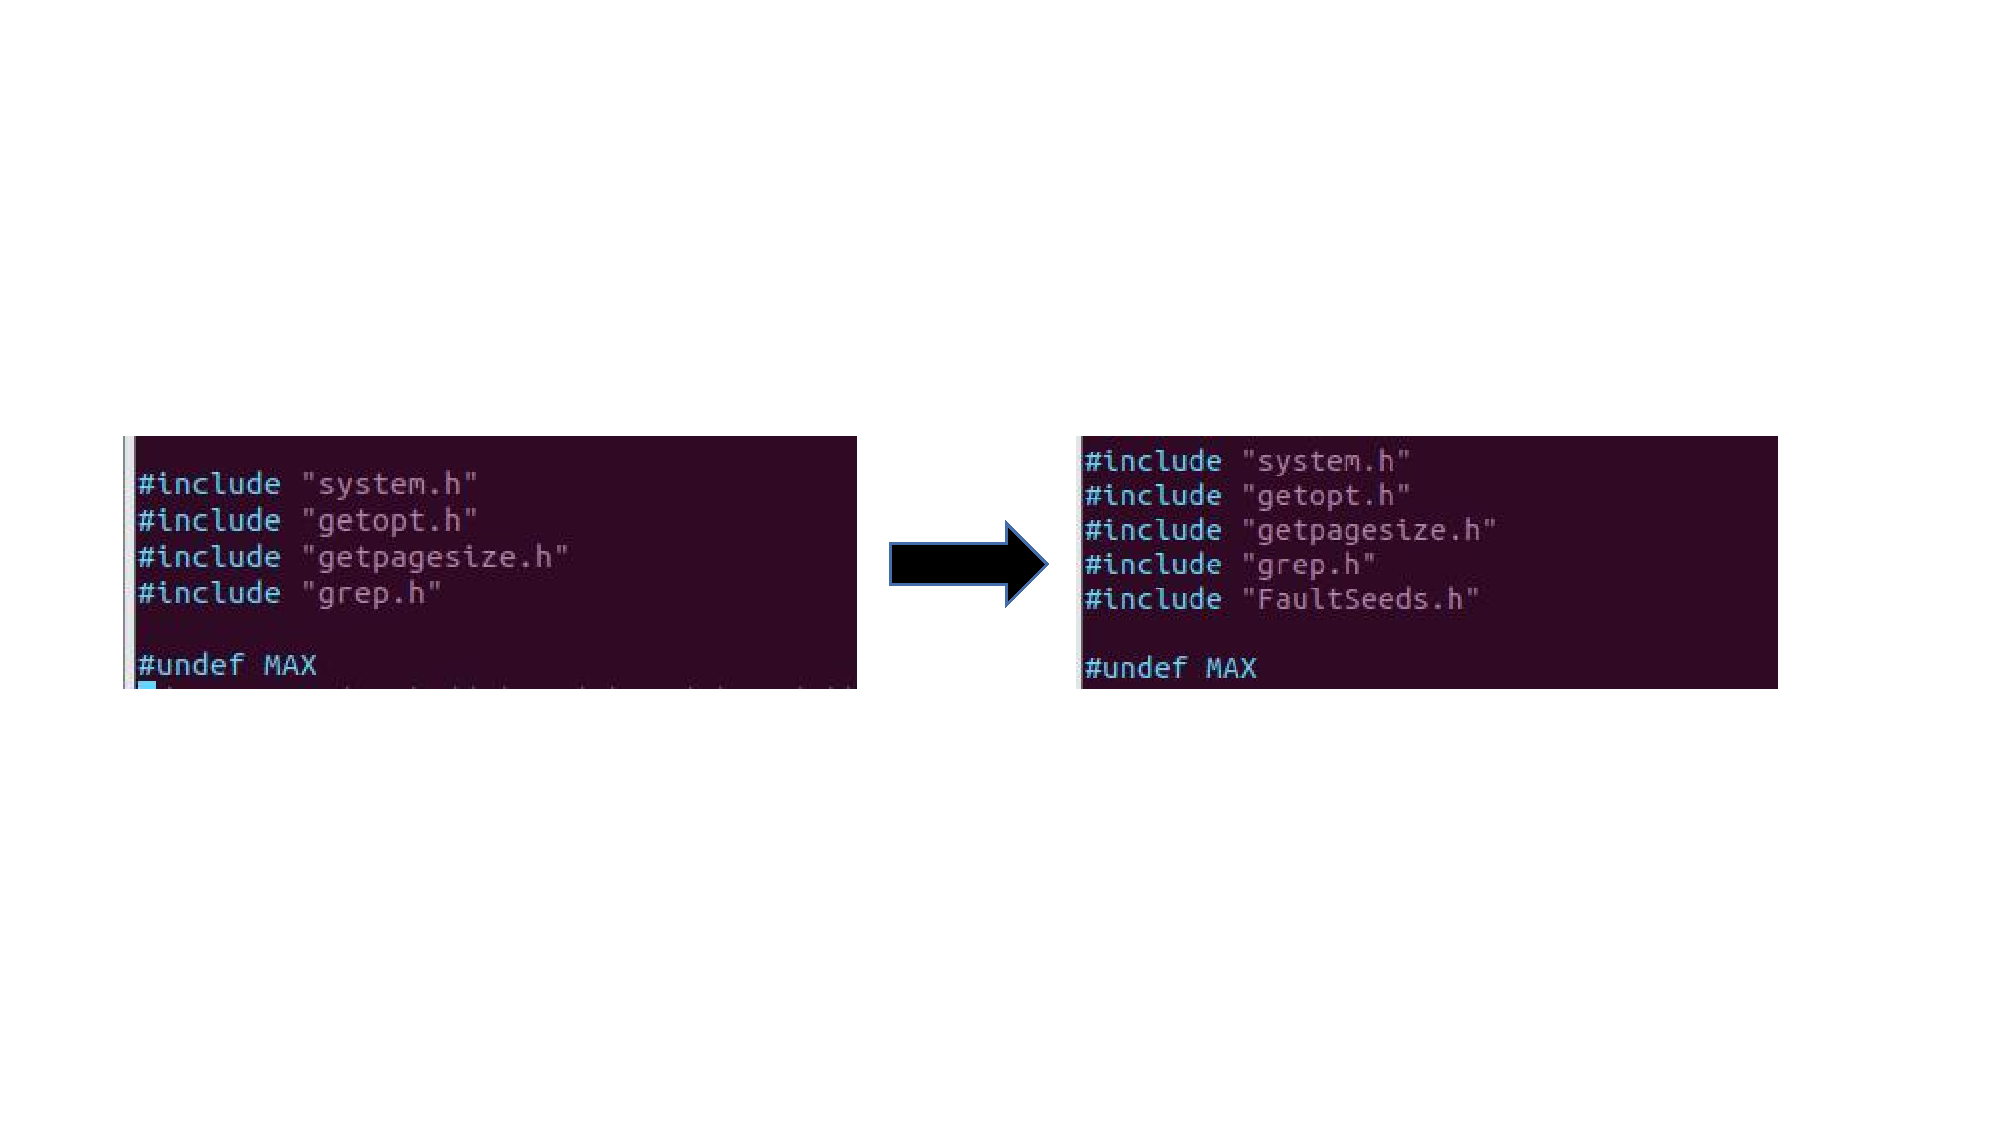
\includegraphics[width=14cm]{images/insert1.pdf}
    \caption{添加$FalutSeeds.h$头文件}
    \label{insert}
\end{figure}

如图\ref{fseed}所示,在$FaultSeeds.h$文件中,存储了18个被注释掉的Bug。在正式的测试过程中,我们需要分别去掉这18行代码的注释来向被测试的程序中植入18个不同的Bug,最后执行含有这些Bug的程序并统计测试用例的通过率。

\begin{figure}[htbp]
    \centering
    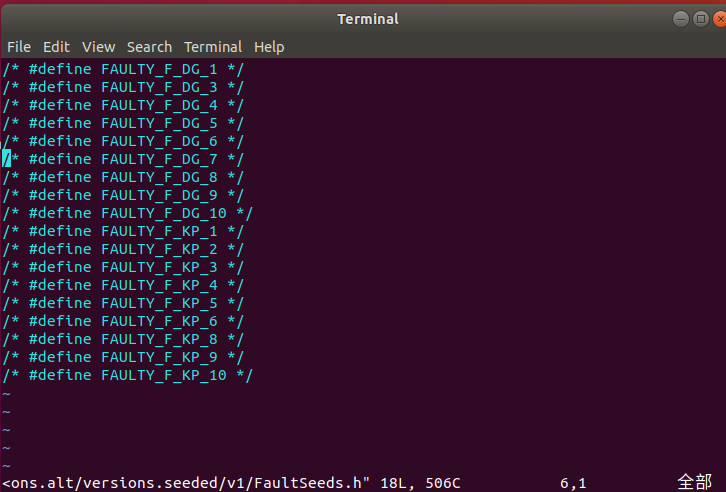
\includegraphics[width=14cm]{images/fseed.png}
    \caption{18个被注释的Bug}
    \label{fseed}
\end{figure}


\subsubsection{预处理代码编写}
考虑到本实验共包含199个测试用例和18个Bug,若手动修改测试用例命令和去除$FaultSeeds.h$中的注释,整个预处理工作将会十分繁琐,因此我们利用Python语言编写代码来自动化预处理过程。

首先,我们对测试用例命令进行修正,如下方代码所示,打开$v0.cov.universe$文件,对其逐行修改:
\begin{lstlisting}[caption={handle.sh pt.2}]
allLines=[]
with open('./grep_1.2/grep/testplans.alt/v1/v0.cov.universe', 'r') as f:
    row=0

    for line in f.readlines():
        allLines.append(line)
        row+=1
        line=line.replace("../inputs","../../../inputs")
        line=line.replace("-P "," ")  # remove "-P "
        line=line.replace("]\n"," ")
        line=line.replace(" ["," ")
        line=line.replace("] "," ")

        line=line.replace("\\","\\\\")   #shell: \\ => \

        line="./grep.exe "+line  #add instruction ./grep.exe
        line=line+" > ./outputs/$i/t"+str(row)+";"   # add output path
        content+=line
\end{lstlisting}
代码解释:
\begin{itemize}
    \item \textbf{修改目录。} 将$../inputs$替换为$../../../inputs$;
    \item \textbf{删除不必要参数及符号。} 将$-P$参数和非测试输入中的中括号删除。注意到测试输入中的中括号前后一定为非空字符,因此替换所有空格及换行符相邻的中括号为空格;
    \item \textbf{处理转义字符。} 由于Python语言中"$\backslash$"同样表示转义,因此Python代码中2个"$\backslash$"对应shell命令中的1个"$\backslash$",4个"$\backslash$"才能表示最终的"$\backslash$"字符本身。
    \item \textbf{添加可执行文件。} 在每行命令的开头添加$./grep.exe$;
    \item \textbf{添加输出路径。} 指定输出路径为$./outputs/\$i/t"+str(row)$,其中$i$为Bug序号,$row$为测试用例序号,即植入第$i$个Bug的情况下,第$row$个测试用例的测试结果。
\end{itemize}

此外,我们编写植入Bug的脚本命令,同时将其和所有修正后的测试用例命令写入同一个脚本文件,这样我们在完成预处理工作的同时也生成了自动执行测试程序的脚本文件$handle.sh$,后续的正式测试过程可以直接运行此脚本得到测试结果。如下所示,$content$初始内容为一些shell命令,并逐行添加修正后的测试用例命令,最终形成正式测试过程所运行的$handle.sh$脚本文件。
\begin{lstlisting}[caption={handle.sh pt.1}]
content="\
    echo 'Lines executed,Branches executed,Taken at least once,Calls executed,' > cov_percentages.csv;\
    mkdir outputs;\
    for((i=1;i<=18;i++));do mkdir ./outputs/$i ;done;\
    sed '' FaultSeeds.h > FaultSeeds;\
    for((i=1;i<=18;i++));\
        do sed $i's#*##g' FaultSeeds > tmp;sed $i's#/##g' \
        tmp > FaultSeeds.h;gcc -fprofile-arcs -ftest-coverage -I. -o grep.exe grep.c;"
\end{lstlisting}
代码解释:
\begin{itemize}
    \item \textbf{创建表头。} 我们将测试出来的代码覆盖率结果写入$cov\_percentages.csv$以便进行统计和分析,此处为统计表格添加表头;
    \item \textbf{创建输出目录。} 所有测试结果输出到$outpus$目录下,$outpus$的每个子目录$i$为第$i$个Bug对应的输出目录。
    \item \textbf{去除注释植入Bug。} 我们利用$sed$命令将对应行的$*$和$/$替换为空字符。另外,我们要执行两次$sed$命令,且$sed$命令替换后的结果不会保存到原文件,因此我们将第一次$sed$后的结果输出到临时文件$tmp$,第二次再输出回到$FaultSeeds.h$文件。每次植入Bug不仅需要去除当前行的代码注释,也需要将上一行的Bug重新加上注释,因此我们在最开始将$FaultSeeds.h$备份到$FaultSeeds$文件,每次去注释植入Bug则基于$FaultSeeds$进行。
    \begin{myquote}
    sed 是一种在线编辑器,处理时,把当前处理的行存储在临时缓冲区中,称为“模式空间”(pattern space),接着用sed命令处理模式空间中的内容,处理完成后,把缓冲区的内容送往屏幕。文件内容并没有改变,因为这些都在模式空间处理
    \footnote{\url{https://www.gnu.org/software/sed/manual/sed.html}}。
    使用sed命令进行替换操作的基本语法格式为:\quad
    \textit{sed 's/目标字符串/替换后的字符串/g' 文件名}

    其中$/$为分隔符,也可以使用\#和@,g表示替换所有的目标字符串,若不添加g则表示只替换第一个匹配的目标字符串。
    \end{myquote}
    \item \textbf{重新编译植入Bug后的程序。} 每次植入Bug后需要重新编译$grep.c$代码,以便可执行文件在对应Bug下执行。
\end{itemize}


\subsection{对正确代码进行测试}
\subsubsection{实验原理}
gcov是一个测试代码覆盖率的工具。与GCC一起使用来分析程序,以帮助创建更高效、更快的运行代码,并发现程序的未测试部分。使用gcov主要完成以下三项工作:
\begin{itemize}
    \item\textbf{在编译阶段产生gcno和gcda文件。}如果需要开启gcov功能,需要在测试开始之前,使用$-fprofile-arcs -ftest-coverage$命令对代码进行插桩。其中$-fprofile-arcs$命令表示在编译时产生gcno文件,它包含了重建基本块图和相应的块的源码的行号的信息。$-fprofile-arcs$命令表示在编译时产生gcda文件,它包含了弧跳变的次数等信息。
    \item\textbf{gcov收集代码运行信息。}首次运行时,会生成gcda文件,记录了代码基本块的执行次数。
    \item\textbf{生成gcov代码覆盖率报告。}利用脚本handle.sh循环运行完测试用例输入并利用gcov命令生成gcov文件,包含了代码覆盖率报告。\footnote{https://blog.csdn.net/yanxiangyfg/article/details/80989680}
\end{itemize}


\subsubsection{数据提取}
观察运行某一条正则表达式的输出结果,如图\ref{grepOutput}所示:

\begin{figure}[htbp]
    \centering
    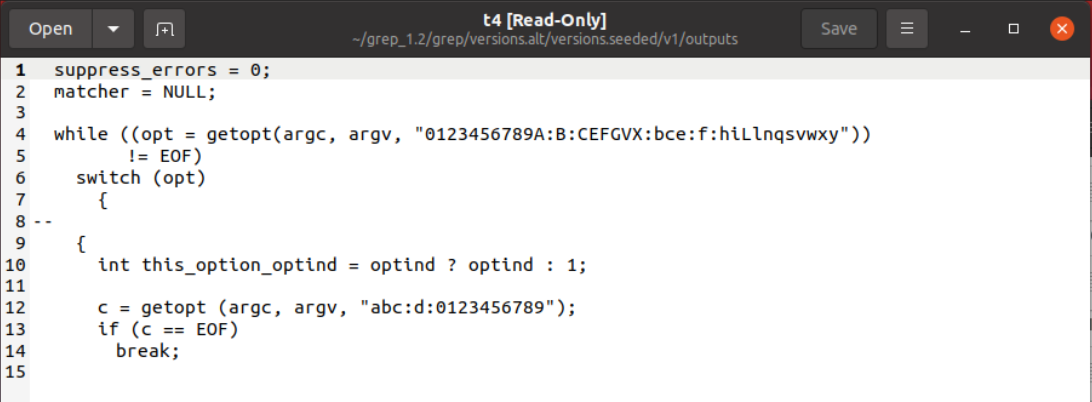
\includegraphics[width=14cm]{images/grepOutput.png}
    \caption{正则表达式的运行结果}
    \label{grepOutput}
\end{figure}

我们可以看到该程序的输出为一串代码。猜测该代码串可能是该程序的输出结果,也可能为翻译某正则表达式的代码。同时也可以知道,该代码串与我们的测试实验关系不大,最终只需使用diff指令判断输出正确与否。

对代码进行测试后,我们得到的结果如图\ref{handleonce1}所示:

\begin{figure}[htbp]
    \centering
    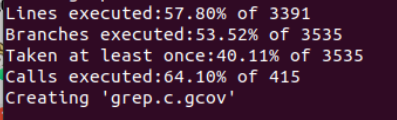
\includegraphics[width=14cm]{images/handleonce1.png}
    \caption{正确代码测试实验结果}
    \label{handleonce1}
\end{figure}

最终代码的语句覆盖率为57.80\%,分支覆盖率为53.52\%,条件覆盖率为40.11\%,函数覆盖率为64.10\%。

我们希望通过shell命令和正则表达式自动化地提取这些数据。我们发现上述数据可以用正则表达式$[0-9].[0-9]\%$表示,且这些数据均不为0.00\%(0.00\%同样能匹配上述正则表达式,且命令行会有这个输出,但它不被我们需要),因此我们使用shell命令grep提取以上数据。具体代码如下:

\begin{lstlisting}[caption={}]
gcov -b grep.c | grep -oE '[0-9]+\.[0-9]+%' | grep -v '0.00' | tr '\\n' ',' >> cov_percentages.csv; echo '' >> cov_percentages.csv;
\end{lstlisting}

代码解释:-o表示只显示匹配pattern的部分,-E表示将pattern当作正则表达式使用,-v表示不匹配0.00, 后续部分表示数据与数据之间使用逗号分隔,语句提取结束后换行。最终将这些数据存储在csv文件中。
\subsubsection{数据可视化}
查阅资料可知,如果在每条测试数据后都对其覆盖率输出,得到的覆盖率为累计覆盖率而不是单个语句的覆盖率。资料如下所示:

\begin{itemize}
    \item 执行计数是累积的。如果在未删除.gcda文件的情况下再次执行示例程序,则源中每行执行次数的计数将添加到上一次运行的结果中。这在几个方面可能很有用。例如,它可用于在测试验证套件的一部分期间累积多个程序运行的数据,或者在大量程序运行中提供更准确的长期信息。
    \item .gcda文件中的数据在程序退出之前立即保存。对于使用-fprofile-arcs编译的每个源文件,分析代码首先尝试读取现有的.gcda文件;如果文件与可执行文件不匹配(基本块计数的数量不同),它将忽略文件的内容。然后,它添加新的执行计数,最后将数据写入文件。
\end{itemize}

我们在测试每条正则表达式后,都对其累计覆盖率进行输出。部分shell命令代码如下所示:

\begin{lstlisting}[caption={}]
./grep.exe  -0 12345 ../../../inputs/grep1.dat  > ./outputs/t1;
gcov -b grep.c | grep -oE '[0-9]+\.[0-9]+%' | grep -v '0.00' | tr '\n' ',' >> cov_percentages.csv; 
echo '' >> cov_percentages.csv;
./grep.exe  -1 12345 ../../../inputs/grep1.dat  > ./outputs/t2;
gcov -b grep.c | grep -oE '[0-9]+\.[0-9]+%' | grep -v '0.00' | tr '\n' ',' >> cov_percentages.csv; 
echo '' >> cov_percentages.csv;
\end{lstlisting}

最终得到覆盖率随样例变化的数据。我们用折线图来表示,如图\ref{handleonce2}所示。

\begin{figure}[htbp]
    \centering
    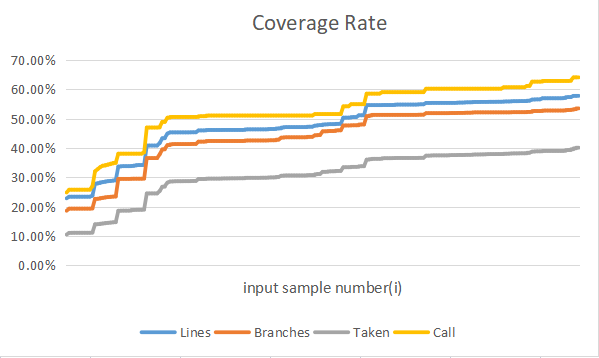
\includegraphics[width=14cm]{images/handleonce2.png}
    \caption{累计覆盖率-样例数目折线图}
    \label{handleonce2}
\end{figure}

从图中可以看出,四种覆盖率的增长具有相同的趋势,且保持函数覆盖率>语句覆盖率>分支覆盖率>条件覆盖率。从增长的缓急方面来看,所有覆盖率在前40个样例时增长较为迅速(有20\%到25\%的提升),而在测试后160个样例时增长缓慢。

\subsection{对植入Bug的代码进行测试}
\subsubsection{实验原理}
grep项目为我们提供了18个bug,它为我们存储在FaultSeeds.h文件中。将注释取消后便可以向代码中植入一个bug。该部分主要是使用gcov命令对植入bug后的代码进行测试,得到其四种覆盖率并对其进行分析。部分实验的shell程序如下所示:

\begin{lstlisting}[caption={}]
# 在根目录建立文件夹outputs存放结果
mkdir outputs;
# 为每一个bug建立一个文件夹存放结果
for((i=1;i<=18;i++));do mkdir ./outputs/$i ;done;
# 用变量FaultSeeds存放文件内容(用于实验结束还原文件)
sed '' FaultSeeds.h > FaultSeeds;
# 移除当前测试bug的‘\’和‘*’(去除注释)
for((i=1;i<=18;i++)); 
do sed $i's#*##g' FaultSeeds > tmp;
sed $i's#/##g' tmp > FaultSeeds.h;
# 插桩,开始测试
gcc -fprofile-arcs -ftest-coverage -I. -o grep.exe grep.c;
............
\end{lstlisting}


\subsubsection{数据提取}
本部分数据提取同样采取grep语句和正则表达式匹配的方法,与4.4部分相同,因此在这里不再赘述。以下为数据提取的结果:

\begin{table}[htbp]
    \centering
    \caption{植入Bug代码的覆盖率} \label{测试表格}
    \begin{tabular}{lcccr}
        \toprule[2pt]
        \textbf{Bug id} & \textbf{Lines executed} & \textbf{Branches executed}  &\textbf{Taken at least once} &\textbf{Calls executed} \\
        \midrule[1pt]
            1 & 57.82\% & 53.52\% & 40.11\% & 64.10\% \\
            2 & 57.82\% & 53.52\% & 40.11\% & 64.10\%\\
            3 & 57.44\% & 53.24\% & 39.75\% & 62.65\%\\
            4 & 57.82\% & 53.52\% & 40.11\% & 64.10\%\\
            5 & 57.82\% & 53.52\% & 40.11\% & 64.10\%\\
            6 & 57.82\% & 53.52\% & 40.11\% & 64.10\%\\
            7 & 57.82\% & 53.52\% & 40.11\% & 64.10\%\\
            8 & 57.84\% & 53.55\% & 40.14\% & 64.10\%\\
            9 & 57.82\% & 53.58\% & 40.11\% & 64.10\%\\
            10 & 57.82\% & 53.50\% & 40.08\% & 64.10\%\\
            11 & 39.85\% & 39.04\% & 26.45\% & 43.37\%\\
            12 & 57.82\% & 53.52\% & 40.11\% & 64.10\%\\
            13 & 57.82\% & 53.52\% & 40.11\% & 64.10\%\\
            14 & 57.68\% & 53.52\% & 40.08\% & 63.13\%\\
            15 & 57.82\% & 53.52\% & 40.11\% & 64.10\%\\
            16 & 57.82\% & 53.52\% & 40.11\% & 64.10\%\\
            17 & 57.82\% & 53.52\% & 40.11\% & 64.10\%\\
            18 & 57.77\% & 53.52\% & 40.11\% & 64.10\%\\
        \bottomrule[2pt]
    \end{tabular}
\end{table}

从表中我们可以看出,除了Bug11之外,其余17个bug的四种覆盖率均与正确情况下相似。而bug11的覆盖率比其余17组数据低了约15-20个百分点。因此,可以猜想bug11错误比较严重,可能在后面diff时有着较高的错误率。

\subsubsection{数据可视化}
对上表中的数据进行可视化展示,可以更加直观的验证上述结论。可视化结果如图\ref{handle}所示。

\begin{figure}[htbp]
    \centering
    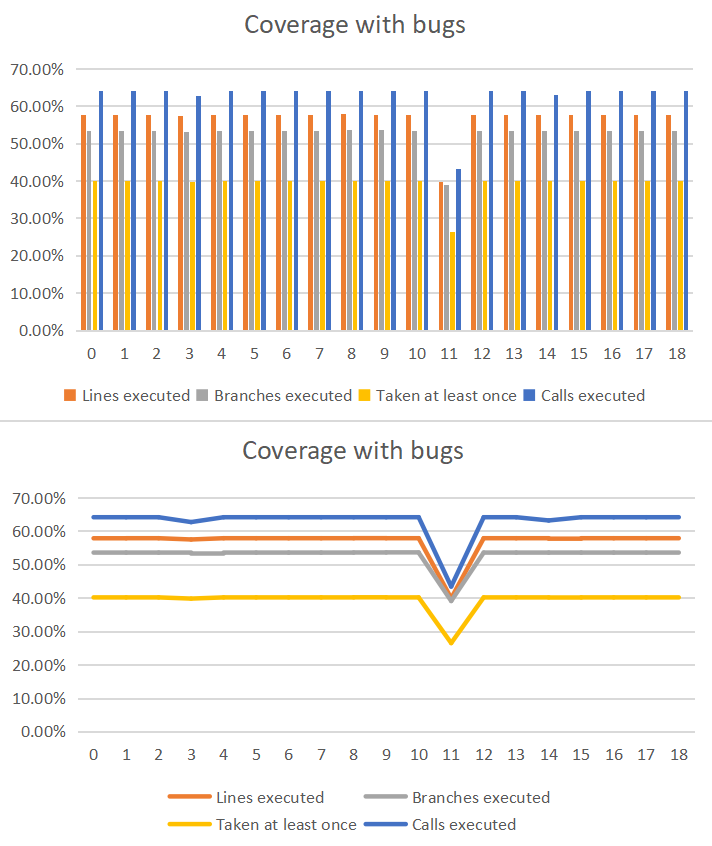
\includegraphics[width=14cm]{images/handle.png}
    \caption{植入Bug后的代码覆盖率}
    \label{handle}
\end{figure}

从表中也可以直观的看出以上结论。其中函数覆盖>语句覆盖>分支覆盖>条件覆盖的结论仍然成立。
\subsection{对正确代码和植入bug代码的测试结果进行比较}


\subsubsection{实验原理}
在生成了正确的结果文件以及分别植入了18个bug的结果文件之后,实验的最后一步是要将分别植入了18个bug的结果文件与正确的结果文件进行比较,从而得知每个bug针对每个测试用例是否通过,若结果一致则说明未检测到bug。

首先我们需要生成一个比较正确版本结果和bug版本结果的脚本文件,使用python编写,具体代码如下:
\begin{lstlisting}[caption={}]
# 新建脚本文件diffAll.sh
with open('diffAll.sh','w') as f:
    #cover the history
    # 写入新建result文件夹的命令
    f.write('mkdir result;\n\
# 写入result文件夹下新建1~18的文件夹的命令
for((i=1;i<=18;i++));do mkdir ./result/$i ;done;\n')

with open('diffAll.sh', 'a') as f:
    # 对于每一个bug版本
    for bugCnt in range(1,19):
        # 生成对应的199个测试结果的比较命令
        f.write(f"echo '---------------------diff bug{bugCnt}--------------------'\n")
        for caseCnt in range(1,200):
            # 比较该bug版本的该测试用例的结果的命令
            f.write(f"echo 'diff case {caseCnt} in {bugCnt}' \n")
            # 将比较结果保存到对应的比较结果文件当中的命令
            f.write(f"diff ./outputs/t{caseCnt} ../../versions.seeded/v1/outputs/{bugCnt}/t{caseCnt} \
                >./result/{bugCnt}/r{caseCnt} \n")
    
    
content="mkdir result; \n\
    for((i=1;i<=18;i++));do mkdir ./result/$i ;done; \n"
\end{lstlisting}

我们用diff命令完成这个比较,将比较后的结果保存到result目录下,然后分析结果是否为空,若为空,则两个文件一致,依次比较完18个版本的输出,写成脚本文件diffAll.sh,生成的部分脚本展示如下:

\begin{lstlisting}[caption={}]
# 建立文件夹result存放比较结果
mkdir result;
# 在result文件夹下为每一个bug建立一个文件夹存放199个结果文件的比较结果
for((i=1;i<=18;i++));do mkdir ./result/$i ;done;
# 对于第一个bug
echo '---------------------diff bug1--------------------'
# 会与第一个bug的第一个测试用例(输入)
echo 'diff case 1 in 1' 
# 比较第一个输入的正确的输出文件
# 和植入了第一个bug的第一个输入的输出文件
# 保存比较结果
diff ./outputs/t1 ../../versions.seeded/v1/outputs/1/t1                 >./result/1/r1 
# 与上一个类似
echo 'diff case 2 in 1' 
diff ./outputs/t2 ../../versions.seeded/v1/outputs/1/t2                 >./result/1/r2 
echo 'diff case 3 in 1' 
diff ./outputs/t3 ../../versions.seeded/v1/outputs/1/t3                 >./result/1/r3 
............
\end{lstlisting}

\subsubsection{数据提取}
在获得了18个bug的199个输入用例与正确结果的比较结果文件之后,需要将每个bug具体对某一个测试用例是否通过的情况提取出来,于是编写了python文件extractDiffData\_per.py,并将结果保存在csv文件中,具体程序如下所示:

\begin{lstlisting}[caption={}]
#每一列代表每一个bug的版本,每一行则为同一个测试用例输入分别到18个bug的版本
with open("dif_percentages_per.csv","w") as f:
    row=["epoch_"+str(bugCnt) for bugCnt in range(1,19)]
    rowStr=",".join(row)
    f.write(rowStr+"\n")

with open("dif_percentages_per.csv","a") as f_csv:
    # 对每一个测试用例
    for caseCnt in range(1,200):
        isFail=[]   # 用来存储各个bug版本是否通过该测试用例
        # 对于每个bug的版本
        for bugCnt in range(1,19):
            filename=f"./result/{bugCnt}/r{caseCnt}"
            # 如果比较结果文件为空,则说明未检测到bug
            if(os.path.getsize(filename)==0):
                isFail.append("0")
            # 比较结果不为空,则说明检测到bug
            else:
                isFail.append("1")
        isFailStr=",".join(isFail)  
        # 将结果写入csv文件中
        f_csv.write(f"{isFailStr}\n")
\end{lstlisting}

为了更好的对比较结果进行分析,我们需要统计出每个bug版本分贝对用通过和未通过的测试用例个数,因此编写了python文件用于进一步提取上一步生成的csv文件当中的数据内容,具体程序如下所示:

\begin{lstlisting}[caption={}]
import os
# 每一列代表每一个bug的版本
# 每一行则为同一个测试用例输入分别到18个bug的版本
with open("dif_percentages_per.csv","w") as f:
    row=["epoch_"+str(bugCnt) for bugCnt in range(1,19)]
    rowStr=",".join(row)
    f.write(rowStr+"\n")

with open("dif_percentages_per.csv","a") as f_csv:
import os
# 生成一个csv文件保存数据提取结果
with open("dif_percentages.csv","w") as f:
    f.write("Bug epoch,Fail case num\n")

# 打开上一步生成的文件
with open("dif_percentages.csv","a") as f_csv:
    # 对于每一个bug版本
    for bugCnt in range(1,19):
        failNum=0   # 统计该bug版本未通过的测试的个数
        # 对每一个测试用例
        for caseCnt in range(1,200):
            # 若文件为空说明通过测试,否则未通过
            filename=f"./result/{bugCnt}/r{caseCnt}"
            if(os.path.getsize(filename)!=0):
                failNum+=1
        # 记录数据         
        f_csv.write(f"{bugCnt},{failNum}\n")
\end{lstlisting}



\subsubsection{数据可视化}
根据上一步得到的数据进行可视化,如图6所示。

\begin{figure}[htbp]
    \centering
    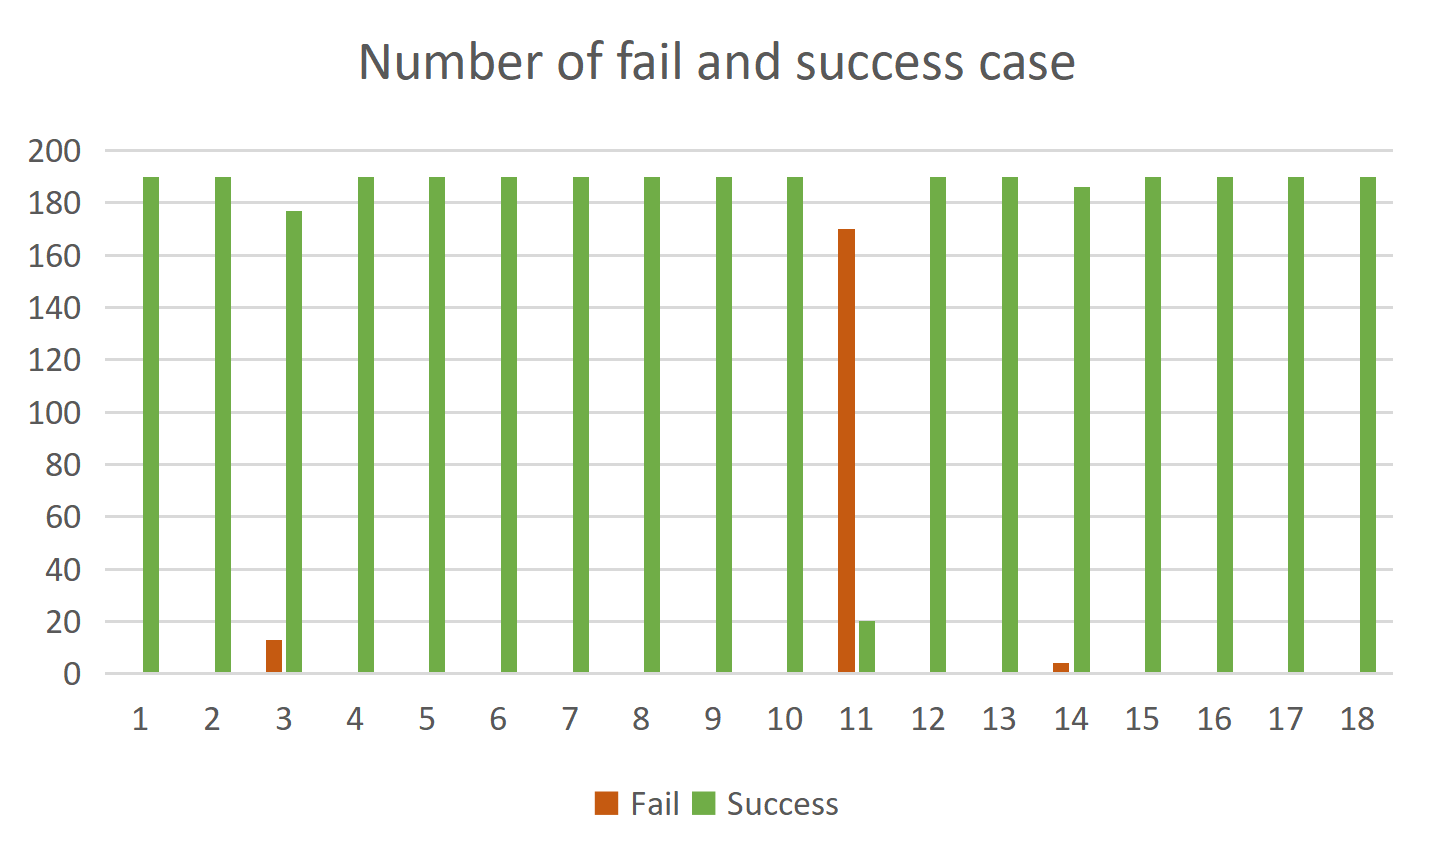
\includegraphics[width=14cm]{images/diff.png}
    \caption{bug版本-通过测试和未通过数目的柱状图}
    \label{allbug}
\end{figure}


由图\ref{allbug}可知,大部分bug版本的程序都通过了所有的测试用例,只有第3和14有极少量测试用例未通过,第11个bug版本有大量测试用例未通过。



\begin{figure}[htbp]
	\centering  %图片全局居中
	\subfigbottomskip=2pt %两行子图之间的行间距
	\subfigcapskip=-5pt %设置子图与子标题之间的距离
	\subfigure[bug3版本的测试用例未通过情况]{
		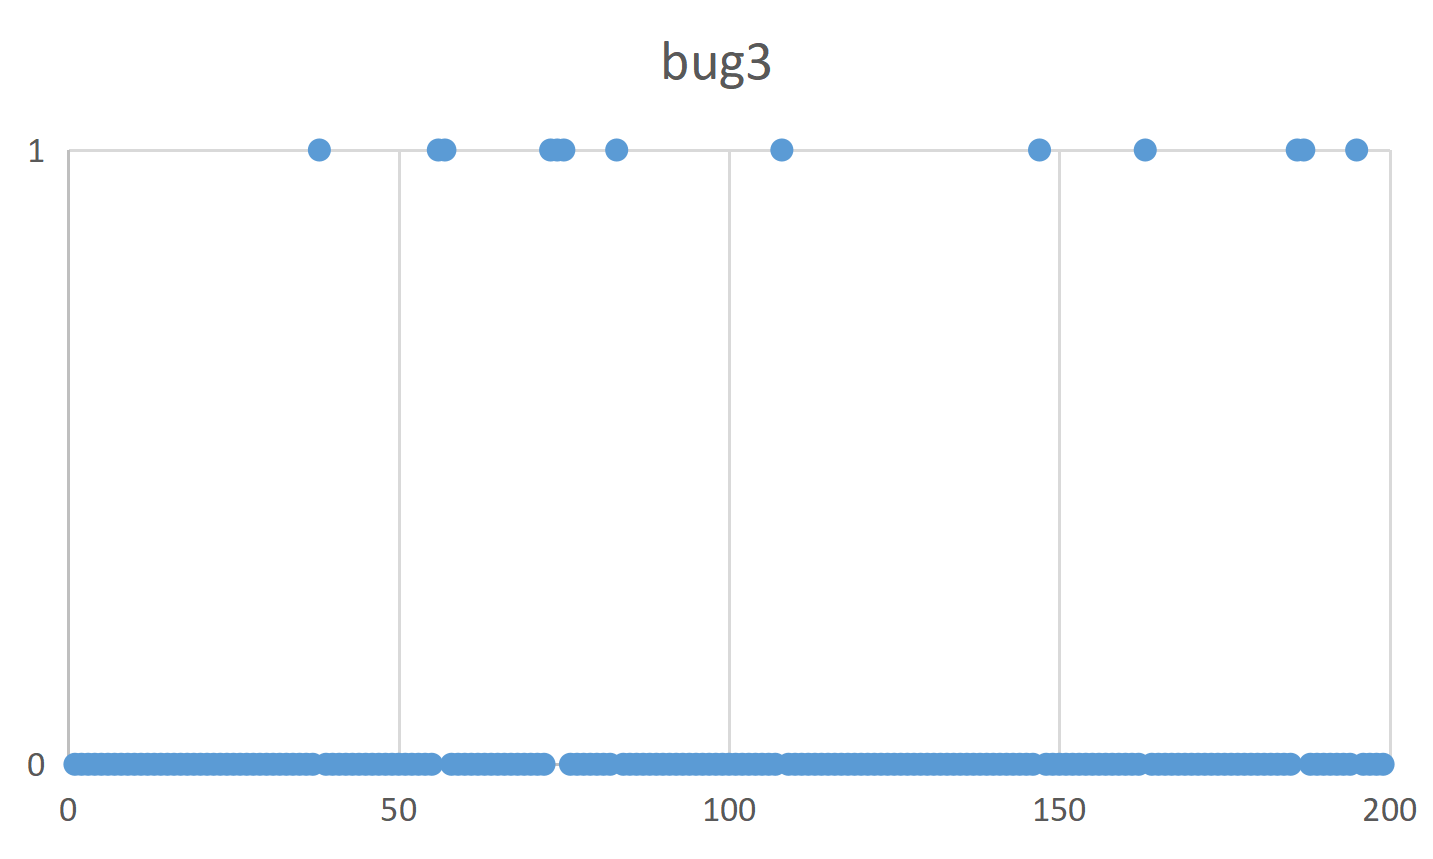
\includegraphics[width=0.48\linewidth]{images/bug3.png}}
	\subfigure[bug14版本的测试用例未通过情况]{
		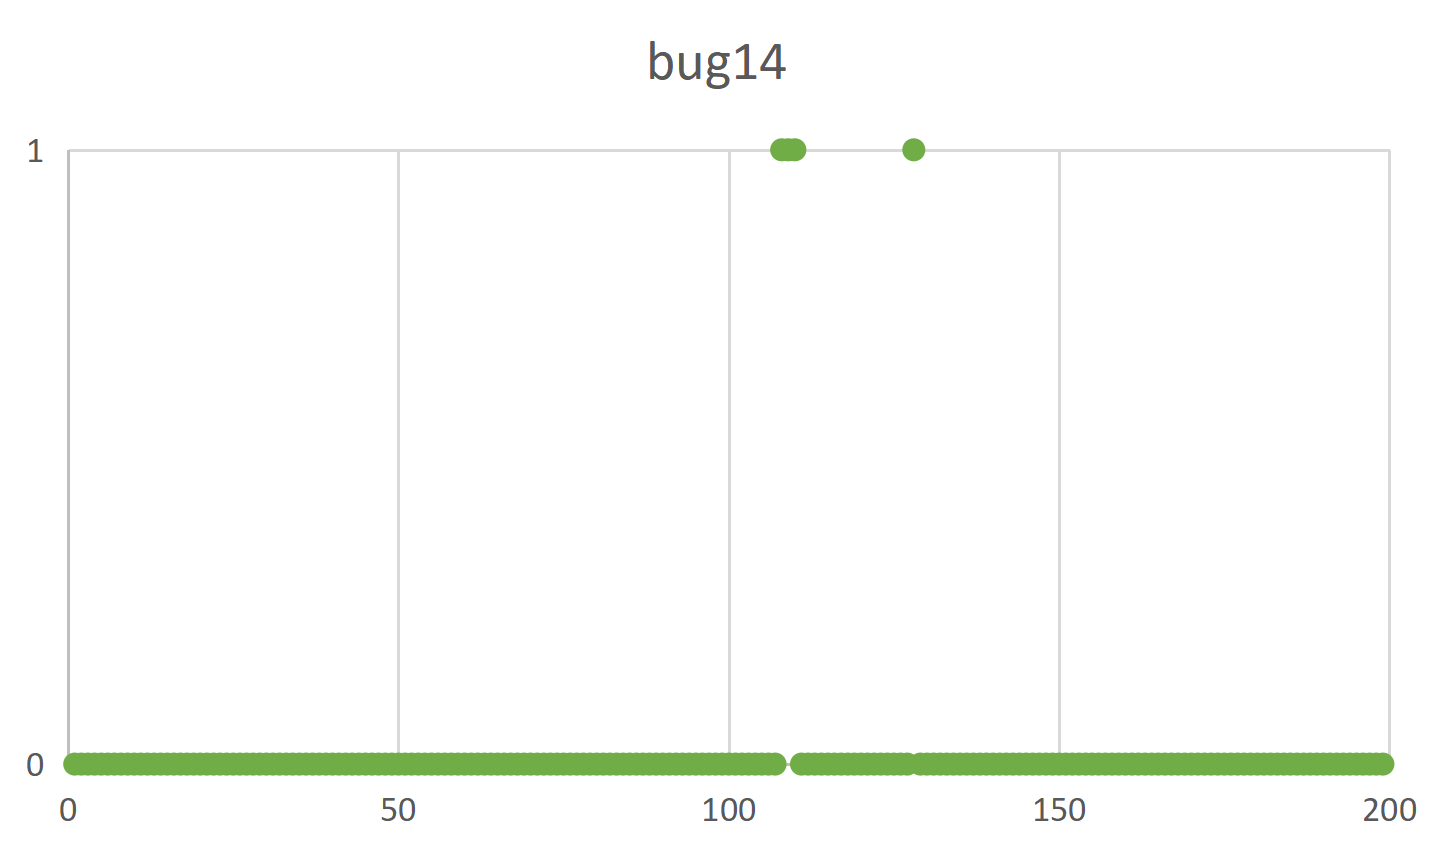
\includegraphics[width=0.48\linewidth]{images/bug14.png}}
	  \\
	\subfigure[bug11版本的测试用例未通过情况]{
		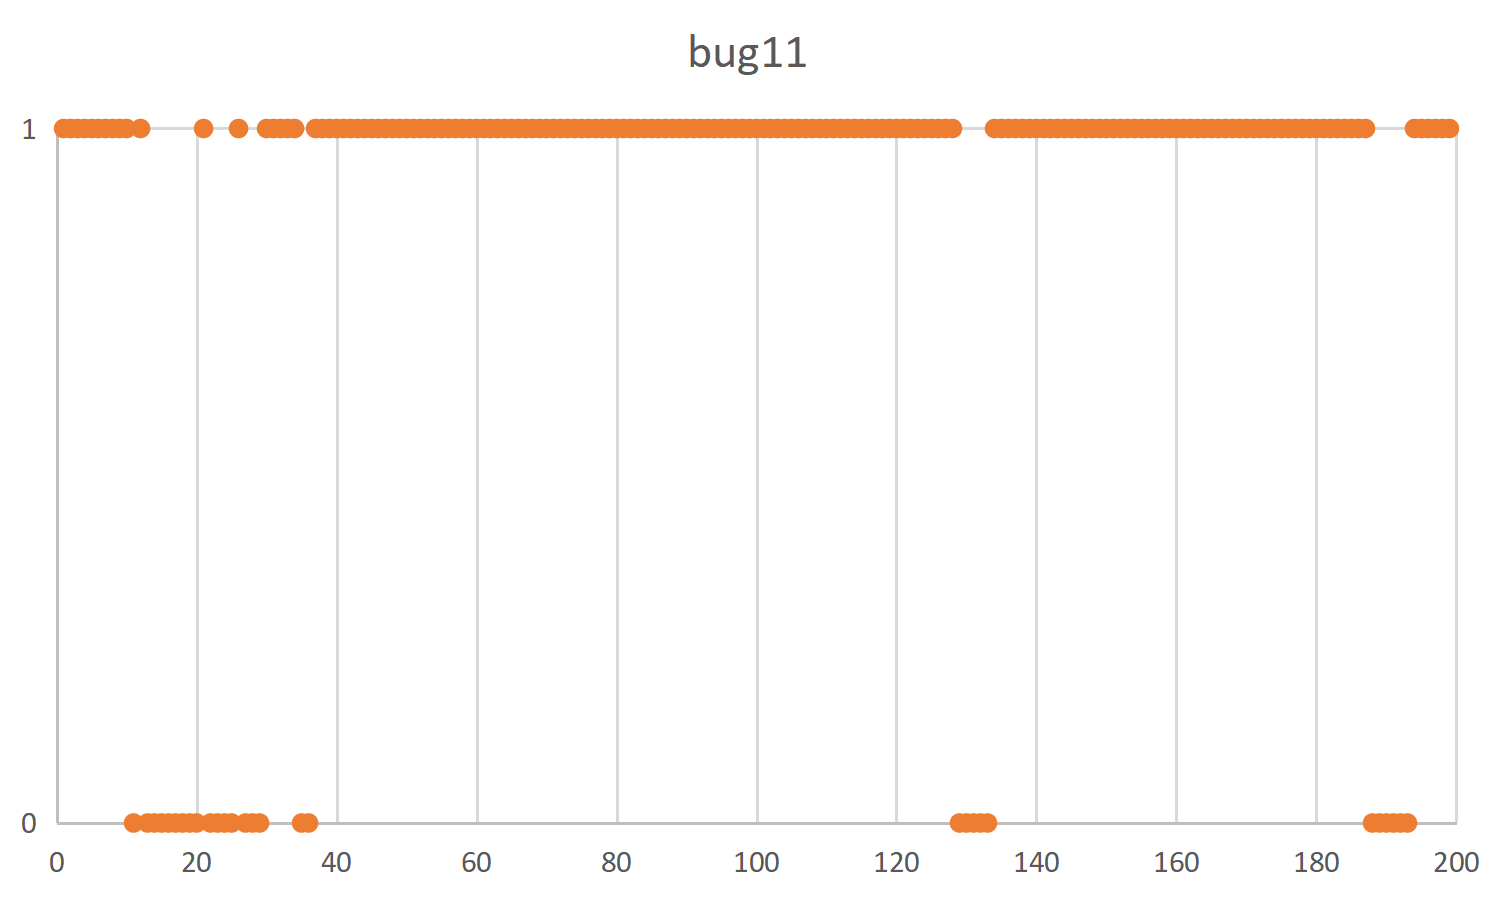
\includegraphics[width=0.8\linewidth=1]{images/bug11.png}}
	%\quad
    \caption{三个有测试用例未通过的bug版本的散点图}
    \label{bugs}
\end{figure}

再分别对第3个、第11个和第14个bug版本的测试用例进行分析,具体结果如图\ref{bugs}所示,图中纵坐标为0表示测试通过,1则表示测试未通过。

具体来说,bug3的版本有13个输入未通过测试,bug11的版本有170个输入未通过测试,bug14的版本有4个未通过测试。


\section{实验总结}
首先我们对实验进行了预处理,包括对测试用例的命令进行修正、将bug进行植入以及编写预处理代码,这里为后面的主要实验部分做好了基础准备,在主要的实验部分,总共有三个核心步骤,分别是对正确代码进行测试、对植入bug的代码进行测试以及对正确代码和植入bug代码的测试结果进行比较。

在对正确的的代码进行测试的部分,我们分别得到了测试的语句覆盖率、分支覆盖率和条件覆盖率。在对植入Bug的代码进行测试部分,我们通过分别对植入bug的头文件进行取消注释来植入每一个bug,最终获得了累计覆盖率以及各个bug版本的三种覆盖率。最后一步就是对正确代码和植入bug代码的测试结果进行比较,通过diff命令我们得到了每个bug版本对于每一个测试用例是否通过的情况,并继续拧了各种角度的数据分析和可视化。


% \subsection{数据分析}
% 把前面三个实验做一个分析总结

% 填充














% \section{参考文献} % 添加一个章节命令
\addcontentsline{toc}{section}{参考文献}
\bibliography{reference}
\bibliographystyle{unsrt}


\addcontentsline{toc}{section}{附录}
\section*{附录}
填充


\end{document}